%%%%%%%%%%%%%%%%%%%%%%%%%%%%%%%%%%%%%%%%%%%%%%%%%%%%%%%%%%%%%%%%%%%%%%%%%%%

\documentclass{standalone}

\usepackage{amsmath}
\usepackage{mathptmx}
\usepackage{pgfplots}
\usetikzlibrary{external}
\tikzexternalize{logarithm}
\pgfplotsset{compat=1.15}

%% IEEE uses Times Roman font, so we'll default to Times.
%% These three commands make up the entire times.sty package.
\renewcommand{\rmdefault}{ptm}
\renewcommand{\ttdefault}{pcr}
\normalfont\selectfont

\begin{document}

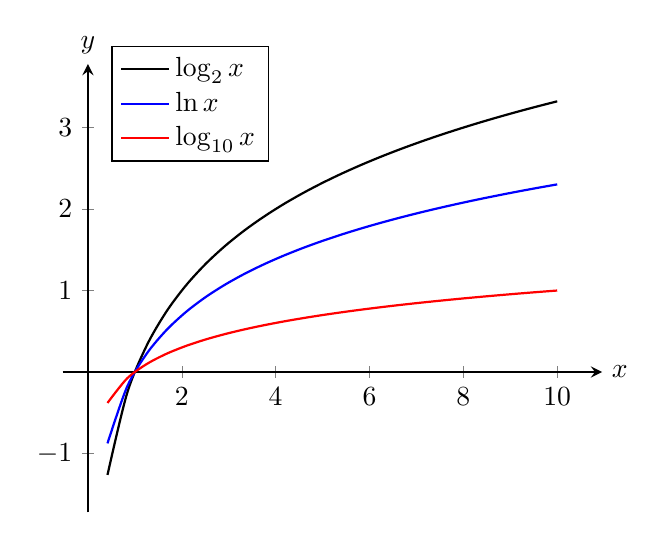
\begin{tikzpicture}
\tikzset{%%
  every mark/.append style={scale=1.0},%%
  scale=1.0%%
}
\pgfplotsset{%%
  every axis/.append style={font=\normalsize}%%
}
%%
\begin{axis}[%%
  axis line style=thick,%%
  axis lines=center,%%
  enlargelimits=true,%%
  legend cell align=left,%%
  legend style={at={(axis cs:0.5,4)},anchor=north west},%%
  plotStyle/.style={%%
    domain=0:10,%%
    mark=none,%%
    smooth,%%
    thick%%
  },%%
  %% x axis
  xlabel={\normalsize $x$},%%
  xlabel style=right,%%
  %% y axis
  ylabel={\normalsize $y$},%%
  ylabel style=above%%
]
%%
%%
%% The binary logarithmic function.
\addplot+ [plotStyle,black]
{log2(x)};
\addlegendentry{$\log_2 x$}
%%
%%
%% The natural logarithmic function.
\addplot+ [plotStyle,blue]
{ln(x)};
\addlegendentry{$\ln x$}
%%
%%
%% The common logarithmic function.
\addplot+ [plotStyle,red]
{log10(x)};
\addlegendentry{$\log_{10} x$}
\end{axis}
\end{tikzpicture}

\end{document}
